\section{Modeling of the \Fermi bubbles at low latitudes}
\label{sec:Modeling}

\begin{comment}
One of the main problems in the analysis of the FBs near the GC is the 
presence of the foreground emission components, 
such as the interactions of cosmic rays with the interstellar gas and radiation fields.
In order to test the possible effects of the foreground emission modeling,
we use several methods to estimate the contribution of the foreground emission to the data.

In particular, there is a tentative
displacement of the FBs to the right of the GC, i.e., negative Galactic latitudes \citep{2016ApJS..223...26A, 2017ApJ...840...43A},
with a spectrum that is harder than the spectrum of the FBs at high latitudes \citep{2017ApJ...840...43A}.
If we assume that the Galactic emission components are approximately symmetric with respect to the GC,
then we can simply mask PS and calculate the difference in gamma-ray flux to the left and to the right from the GC.
The difference should be approximately equal to the asymmetric part of the FBs emission
under the assumption that the other Galactic components and unresolved PS are symmetric with respect to the GC
(Section \ref{sec:data_diff}).

In order to further test the hypothesis of the asymmetric and hard emission from the FBs at low latitudes,
we use the data at energies $\lesssim \SI{1}{GeV}$ to create a template of the Galactic emission,
provided that the expected contribution of the FBs at these energies is small relative to the rest of the Galactic components.
Then we fit the template derived from the low-energy data together with an isotropic template at higher energies
outside of the FBs area.
The FBs intensity is determined by extrapolating the model inside the FBs area using the full template and by subtracting the model
from the data (Section \ref{sec:le_data_model}).
As an alternative approach, instead of fitting outside of the FBs area, we add to the model independent flat rectangular templates with the size
approximately following the FBs size and fit the model over the whole sky.
The flux attributed to these rectangular templates is used as an estimate of the average flux in the FBs in the corresponding areas
(Section \ref{sec:box_model}).

We also calculate the flux attributed to the bubbles using one of the diffuse emission models from \citep{2017ApJ...840...43A}
(Section \ref{sec:galprop_model}).

\end{comment}

\subsection{East-west  asymmetry in the data}
\label{sec:data_diff}

In order to investigate the tentative asymmetry of the emission at the base of the FBs relative to the GC, 
we compare the \Fermi-LAT data east and west of the GC. 
We mask the 200 brightest above 1 GeV point sources (PS) in the Third \Fermi-LAT source catalog \citep[3FGL,][]{2015ApJS..218...23A}
with a circle of radius $\frac{\delta}{\sqrt{2}} + 0^\circ\!\!.5$, where $\delta = 0\degr\!\!.46$ is the characteristic size of the pixels
so that ${\delta}/{\sqrt{2}}$ is half of the pixel diagonal (if it were a square), while $0\degr\!\!.5$ is comparable to 68\% containment
above $\approx 2$ GeV.
In order to avoid possible bias by masking more pixels on one side of the GC,
we symmetrize the PS mask relative to the GC, i.e., we put $m_{-b, -\ell} = 0$ if $m_{b, \ell} = 0$ and vice versa.
This PS mask is also used in the following sections (apart from Section \ref{sec:galprop_model}).
The data is averaged over regions to the west ($0^\circ < \ell < 10^\circ$) and to the east ($-10^\circ < \ell  <  0^\circ$) 
of the GC at different latitudes. 
The regions have a latitude width of $4^\circ$. 
%$10^\circ$ for $b >|10^\circ|$ and a width of  $4^\circ$ for  $b <|10^\circ|$. 
The fraction of masked pixels is about 50\% within $|b| < 2^\circ$, about 10\% for $2^\circ < |b| < 6^\circ$, and less than  5\% 
for $|b| > 6^\circ$.

The difference of the averaged intensity of emission west minus east of the GC is shown in Fig. \ref{fig:data_diff}. 
The error bars represent the statistical errors.
At high latitudes, $b >|10^\circ|$, the emission is relatively symmetric. 
The emission for latitudes $b \in (-6^\circ, -2^\circ)$ and $b \in (-2^\circ, 2^\circ)$ shows excess emission to the west of the GC, 
which remains significant at high energies. 
There is also asymmetry in the opposite direction for $b < 6^\circ$ (east is brighter than west), which is due to the cocoon inside the 
southern lobe of the FBs \citep{2012ApJ...753...61S, 2014ApJ...793...64A}.
The Fermi-LAT exposure within $|b| < 10^\circ$ and $|\ell| < 10^\circ$ is rather uniform, 
the maximal fractional variation of the exposure in this region for $E > 1$ GeV is less than 4\%.

\begin{figure}[h]
\centering
 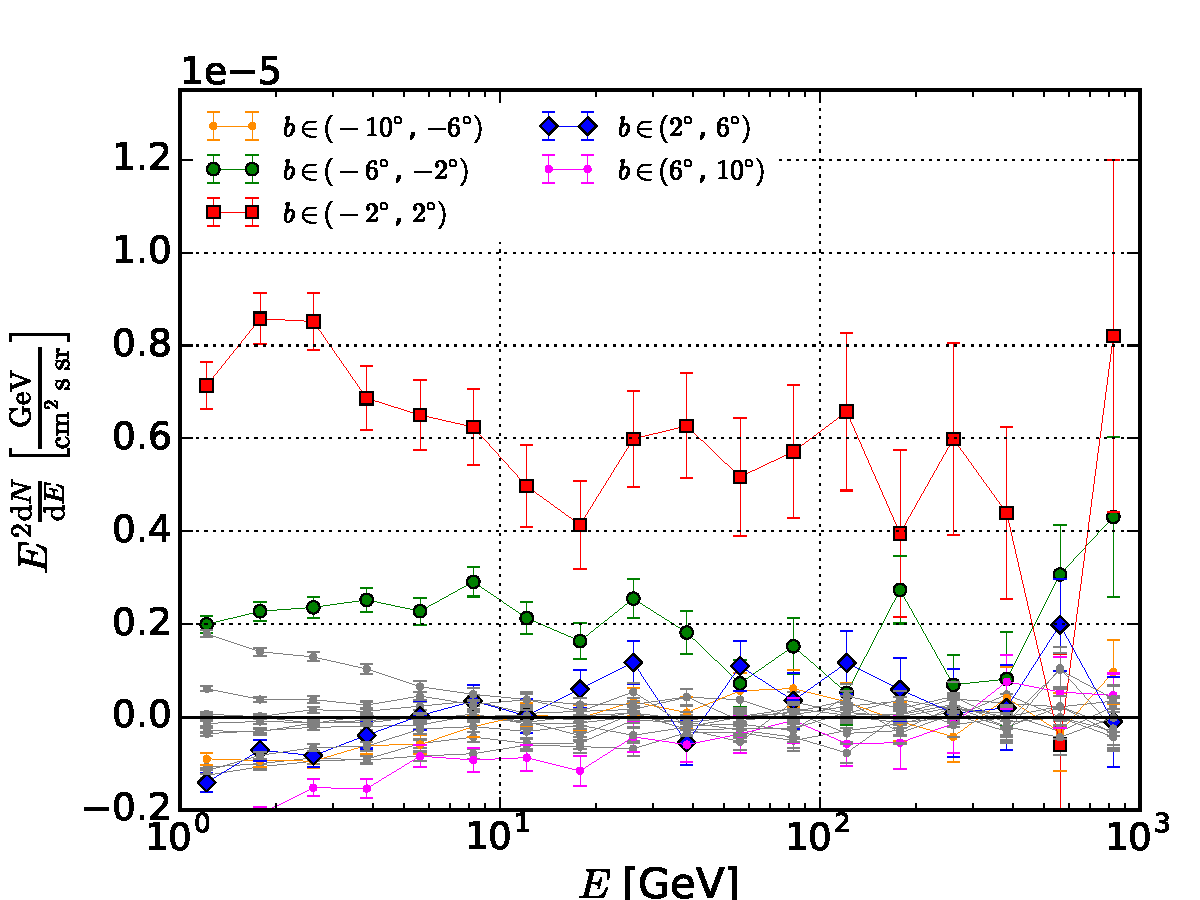
\includegraphics[width=0.5\textwidth]{plots/Difference_data_for_different_latitudes.pdf}
 \caption{Difference west minus east in the \Fermi-LAT intensity relative to the GC after masking bright PSs.
 The PS mask is symmetrized relative to the GC.
 The west (east) region is defined between $-10^\circ < \ell <0^\circ$ ($0^\circ < \ell <10^\circ$).
 Grey lines show spectra for latitudes $|b| > 10^\circ$. 
 }
 \label{fig:data_diff}
\end{figure}

\subsection{Low-energy data as a background model}
\label{sec:le_data_model}

\begin{figure*}[t]
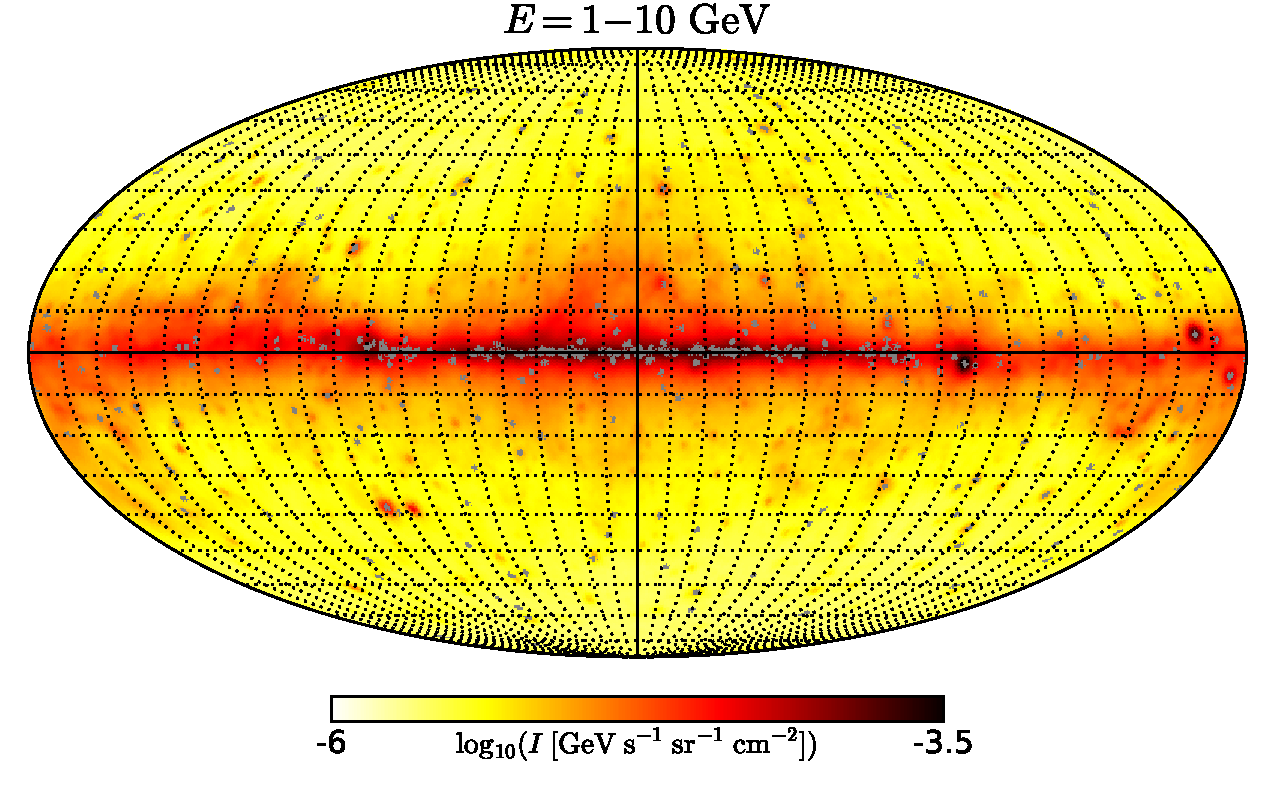
\includegraphics[width=0.33\textwidth]{plots/Mollweide_LowE_model_03-10GeV_flux_source_range_0_log.pdf}
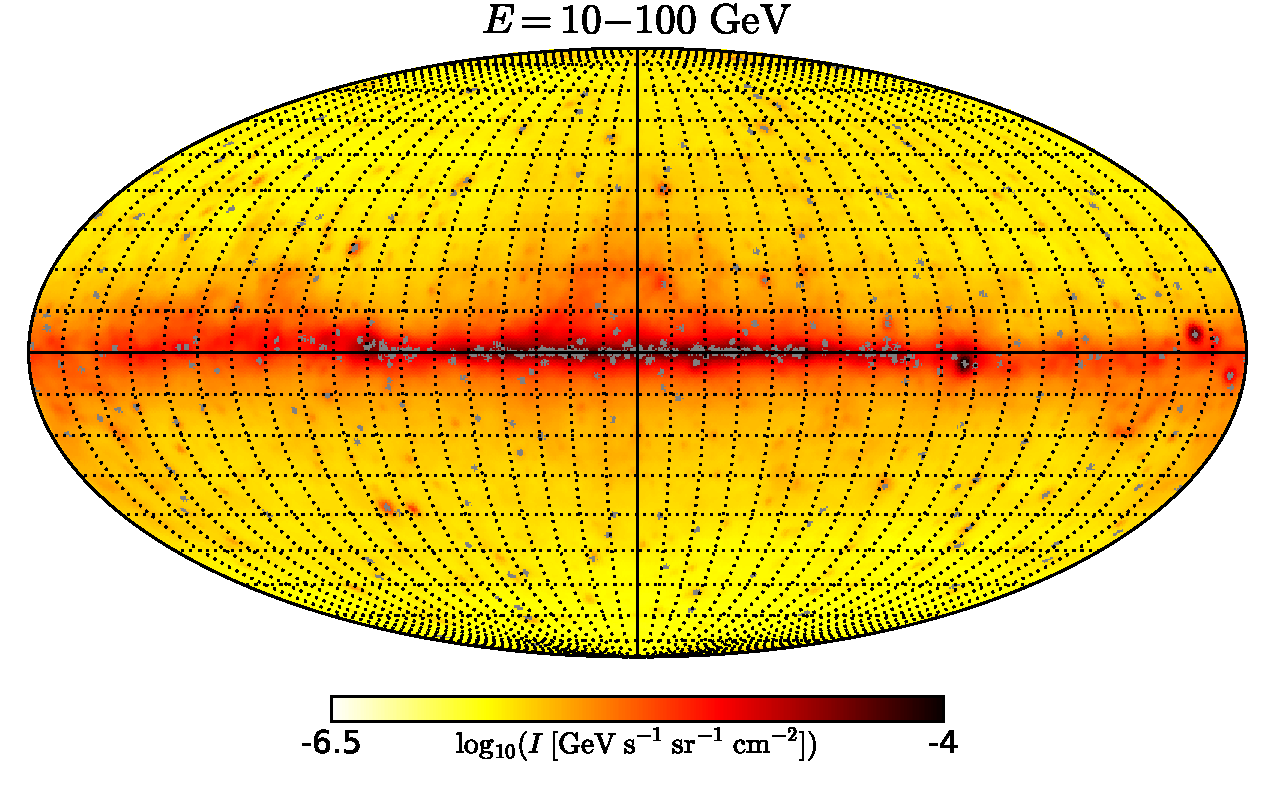
\includegraphics[width=0.33\textwidth]{plots/Mollweide_LowE_model_03-10GeV_flux_source_range_1_log.pdf}
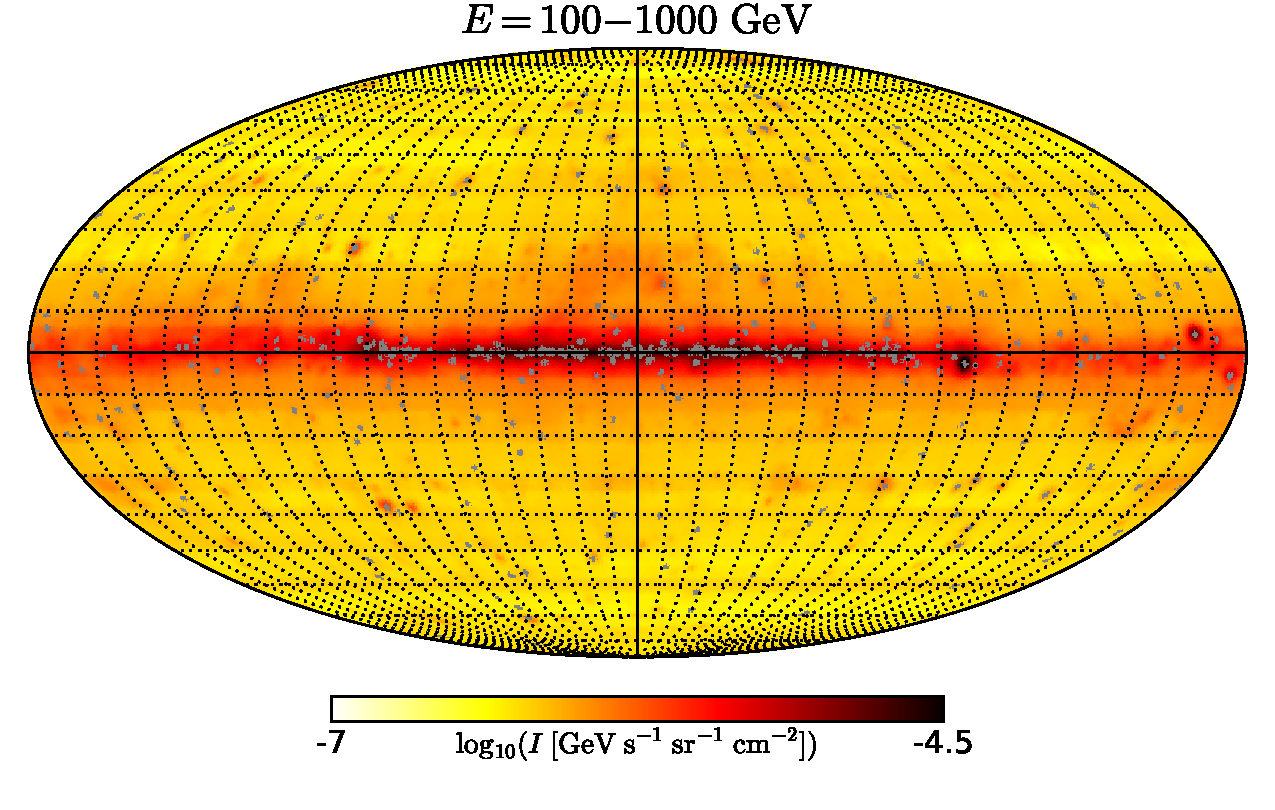
\includegraphics[width=0.33\textwidth]{plots/Mollweide_LowE_model_03-10GeV_flux_source_range_2_log.pdf}
\caption{Energy flux of the diffuse emission model based on the low-energy data (Section \ref{sec:le_data_model})
integrated over three energy ranges. }
\label{fig:Maps_lowE_model}
\end{figure*}


\begin{figure*}[t]
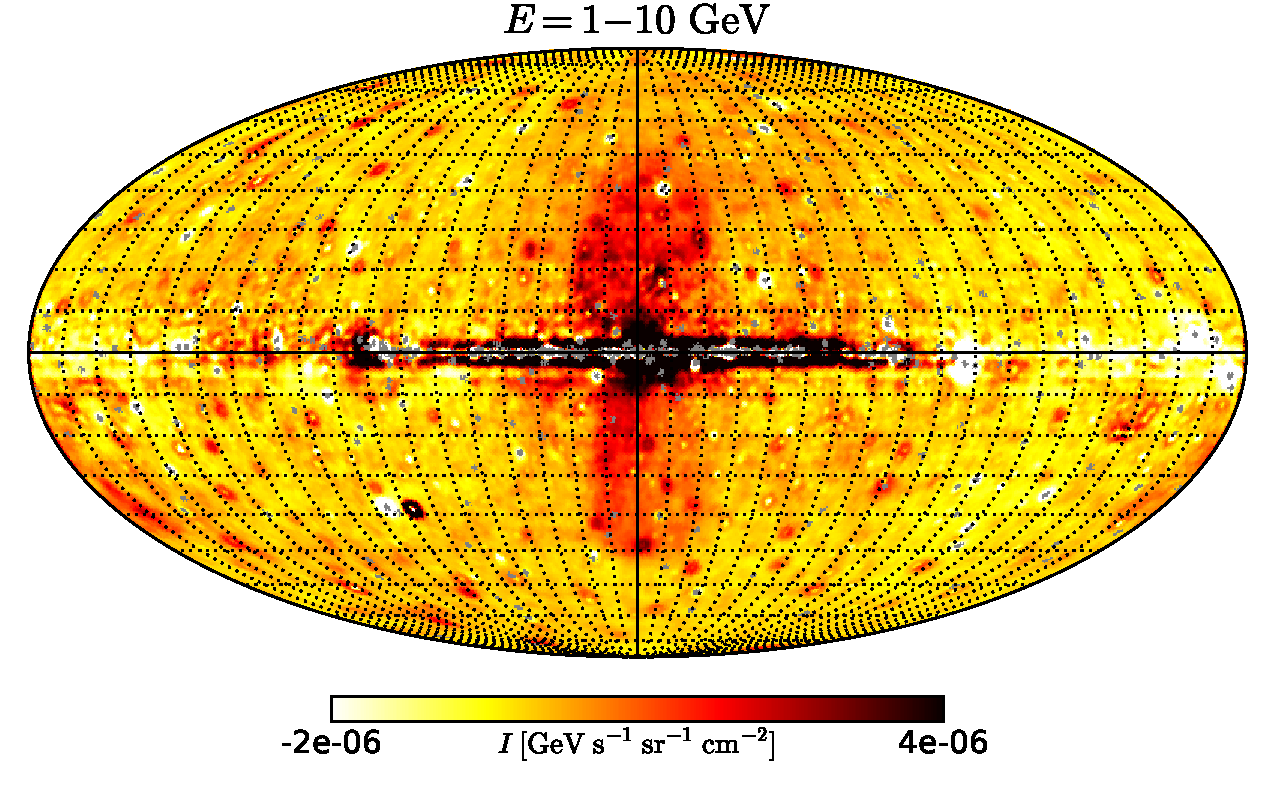
\includegraphics[width=0.33\textwidth]{plots/Mollweide_LowE_03-10GeV_flux_source_range_0.pdf}
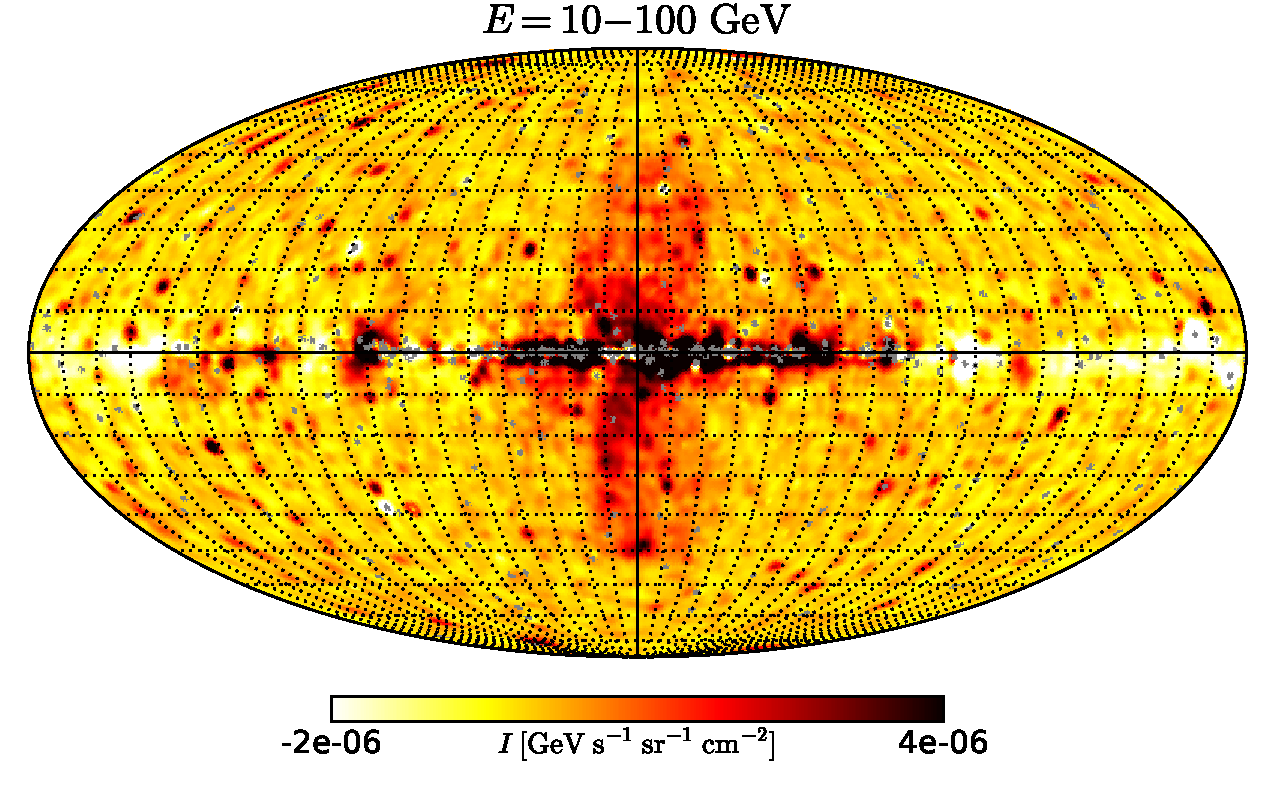
\includegraphics[width=0.33\textwidth]{plots/Mollweide_LowE_03-10GeV_flux_source_range_1.pdf}
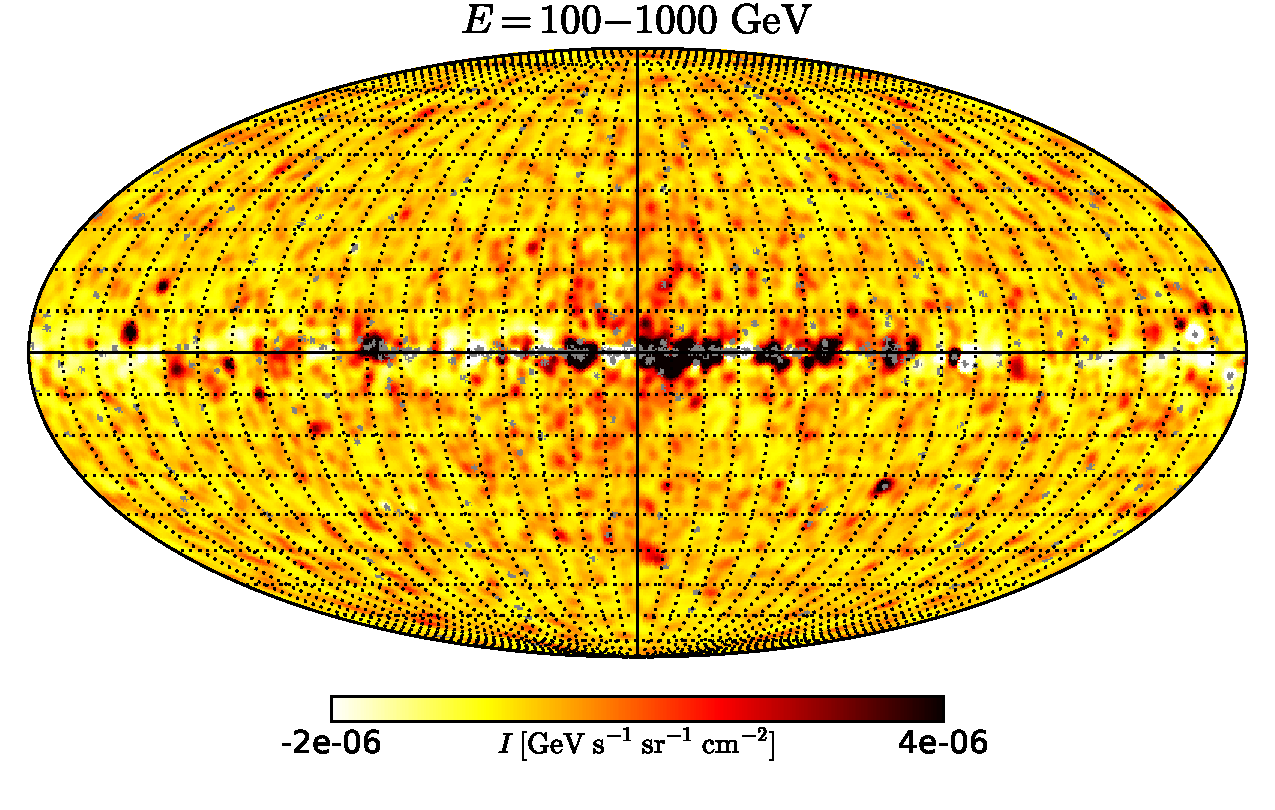
\includegraphics[width=0.33\textwidth]{plots/Mollweide_LowE_03-10GeV_flux_source_range_2.pdf}
\caption{Energy flux of the residuals of the low-energy model derived in Section \ref{sec:le_data_model}
integrated over three energy ranges. }
\label{fig:Maps_lowE}
\end{figure*}


In the previous section we have shown that the west-minus-east difference in the \Fermi-LAT data in the Galactic plane relative to the GC has a hard 
spectrum $\sim E^{-2}$ up to 1 TeV.
One of the simplest ways to separate the soft component of emission from the hard one is to use the low-energy data as
a model of the soft component and subtract it from the data at higher energies.
Gamma rays produced in interactions of the stationary Galactic population of CR with gas and ISRF,
i.e., the $\pi^0$, bremsstrahlung, and IC components,
dominate the gamma-ray emission in the Galactic plane in the energy range $E \lesssim \SI{1}{GeV}$. 
Consequently, the low-energy \Fermi-LAT data is a good tracer for diffuse gamma-ray emission in the Galactic plane and can be used to create a spatial template for the Galactic foreground.
The 68\% containment for the \Fermi-LAT photons between $\SI{316}{MeV}$ and $\SI{1}{GeV}$ (averaged with $E^{-2}$ spectrum) is about $1^\circ\!\!.5$,
which is much larger than the sub-degree angular resolution above $\SI{1}{GeV}$.
In order to compensate for the difference in the angular resolution, 
we smooth the data in each high-energy bin above 1 GeV
with a Gaussian kernel of $\sigma = \ang{1}$ (which corresponds to $68\%$ containment angle of
$1^\circ\!\!.5$ in 2 dimensions).%
\footnote{In general, the width of the Gaussian kernel $\sigma$ can be obtained by subtracting in quadrature
the equivalent widths at low and at high energies $\sigma^2 = \sigma_{\rm low}^2 - \sigma_{\rm high}^2$.
Since $\sigma_{\rm low}^2 \gg \sigma_{\rm high}^2$, we neglect $\sigma_{\rm high}^2$ and smooth the 
data at high energies with $\sigma_{\rm low} = 1^\circ$.}

We separate the whole sky in latitude stripes of $\ang{4}$ width where the \Healpix pixels are assigned to stripes that contain the centers of the pixels.
We parametrize the model in each stripe and each energy bin independently, i.e., 
in the latitude stripe $b$ and energy bin $E$ the model consists of two terms:

\be
\lb{eq:le_model}
N^\model_{b}(E, i) = k_{b}(E) \cdot \tilde N^\low_{b}(E, i) + c_b(E) \cdot \tau(E, i),
\ee
where $i$ is the pixel index,
$k_{b}(E) \cdot \tilde N^\low_b(E, i)$ is proportional to the low-energy photon counts summed over 
$n_\low = 3$ energy bins between between $\SI{316}{MeV}$ and $\SI{1}{GeV}$ 
rescaled by the ratio of exposures at low and at high energies:

\be
\tilde N^\low_b(E, i) = \frac{1}{n_\low} \left(\sum_{\epsilon \in (0.3 - \SI{1.0}{GeV})} \frac{N^\low(\epsilon, i)}{\tau(\epsilon, i)}\right) \cdot \tau(E, i).
\ee
The term $c_b(E) \cdot \tau(E, i)$ in Equation (\ref{eq:le_model}) is proportional to the exposure $\tau(E, i)$: it accounts for the isotropic extragalactic background and partially compensates for the latitude dependent IC emission. 

We determine the parameters $c_{b}(E)$ and $k_{b}(E)$ by fitting the model to the \Fermi-LAT data in energy bins $E > \SI{1.0}{GeV}$.
We maximize the log likelihood of the gamma distribution 
with respect to parameters $c_{b}(E)$ and $k_{b}(E)$
using the Python iminuit optimizer%
\footnote{
Since the smoothed data has non-integer values, 
we use the gamma distribution $p(x; \td{k} + 1) = \frac{x^{\td{k}}}{\G (\td{k} + 1)}e^{-x}$ instead of the Poisson distribution, 
where $\td{k}$ is the value in the smoothed photon counts map (see Appendix \ref{app:gamma}).
For an unsmoothed map, $\td{k}$ would be the observed number of photons in a pixel.
}.
In order to avoid an overcompensation 
for the flux from the FBs, the region $-20^\circ < \ell < 20^\circ$
is excluded from the fit, i.e., the fit is performed for 
the total remaining length of the stripe $20^\circ < \ell < 340^\circ$.
In the following, the region $-20^\circ < \ell < 20^\circ$ will be refered to as the FBs region of interest (ROI).
PSs are masked with the mask described in Section \ref{sec:data_diff}.

%\red{Dima: do we symmetrize the PS mask in the analysis as well, not only in the calculation of the asymmetry in the data?}

After we fit the model in each latitude stripe, we interpolate it inside the bubbles ROI.
The intensity of the model energy flux integrated in three energy ranges
is shown in Figure \ref{fig:Maps_lowE_model},
while the residuals after subtracting the model from the data are presented in Figure \ref{fig:Maps_lowE}.
The FBs are clearly visible in the first two energy ranges, $E = 1 - \SI{10}{GeV}$ and $E = 10 - \SI{100}{GeV}$.
For $E = \SI{100}{GeV} - \SI{1}{TeV}$ the statistics is low, but one can still see an excess near the GP.
There are other regions of large residuals, mostly in the Galactic plane, but also some PS at high latitudes.
These are diffuse and point-like sources with spectra harder than the average spectra of Galactic and
extragalactic sources.

\subsection{Rectangles model of the bubbles}
\label{sec:box_model}

In the previous subsection, we exclude the ROI of the FBs.
In this subsection, we perform the fit over the whole sky and model the emission from the FBs using rectangles of small size.
%Our first simple ansatz for a model of the FBs consists of rectangular templates that approximately cover the area of the FBs. 
In order to explore the east-west asymmetry of the FBs, 
we introduce two rectangular templates in each latitude stripe $b$ and energy bin $E$: 
one east, $\ell \in (-20^\circ, 0^\circ)$, and one west, $\ell \in (0^\circ, 20^\circ)$, of the GC.
The width of the rectangles is $4^\circ$, i.e., the same as the width of the latitude stripes.
%Below $|b| = 10^\circ$, the width of the rectangles is $4^\circ$ with centers at $b = 0^\circ,  \pm 4^\circ,  \pm 8^\circ$,
%while above $|b| = 10^\circ$ the width is $10^\circ$ with centers at $b = \pm 15^\circ,  \pm 25^\circ,  \ldots, \pm 55^\circ$.
We use the same foreground model as in Section \ref{sec:le_data_model} plus the isotropic template.
Overall, the model has four terms in each energy bin:

\be
\begin{split}
N^\model_{b}(E, i) &= k_{b}(E) \cdot \tilde N^\low_{b}(E, i) + c_b(E) \cdot \tau(E, i)\\
&\quad + R^\east_b(E) + R^\west_b(E).
\end{split}
\ee
where the scaling parameters $k_{b}(E)$, $c_{b}(E)$, $R^\east_b(E)$, and $R^\west_b(E)$ are determined independently 
in each $4^\circ$ latitude stripe and in each energy bin $E > 1$ GeV
by  fitting the model to the smoothed \Fermi-LAT data.
The energy fluxes of the model and the residuals integrated for $E = 10 - \SI{100}{GeV}$ are shown in Fig. \ref{fig:Maps_Rectangles}.
%Here we plot the sum of the residual and the rectangles model.
%With residual we denote the sum of the rectangles-model residual and the rectangles template in the following.

\begin{figure}[h]
\centering
 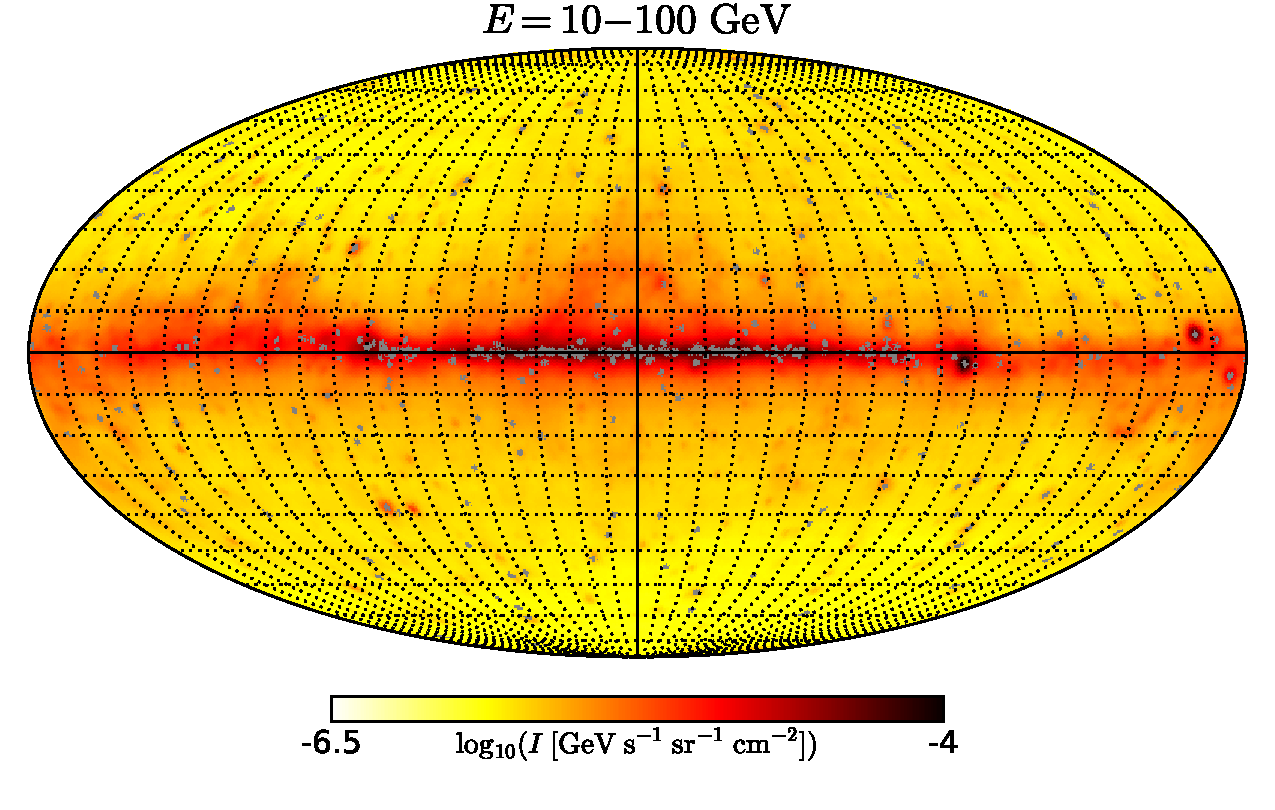
\includegraphics[width=0.45\textwidth]{plots/Mollweide_Boxes_model_03-10GeV_flux_source_range_1_log.pdf}
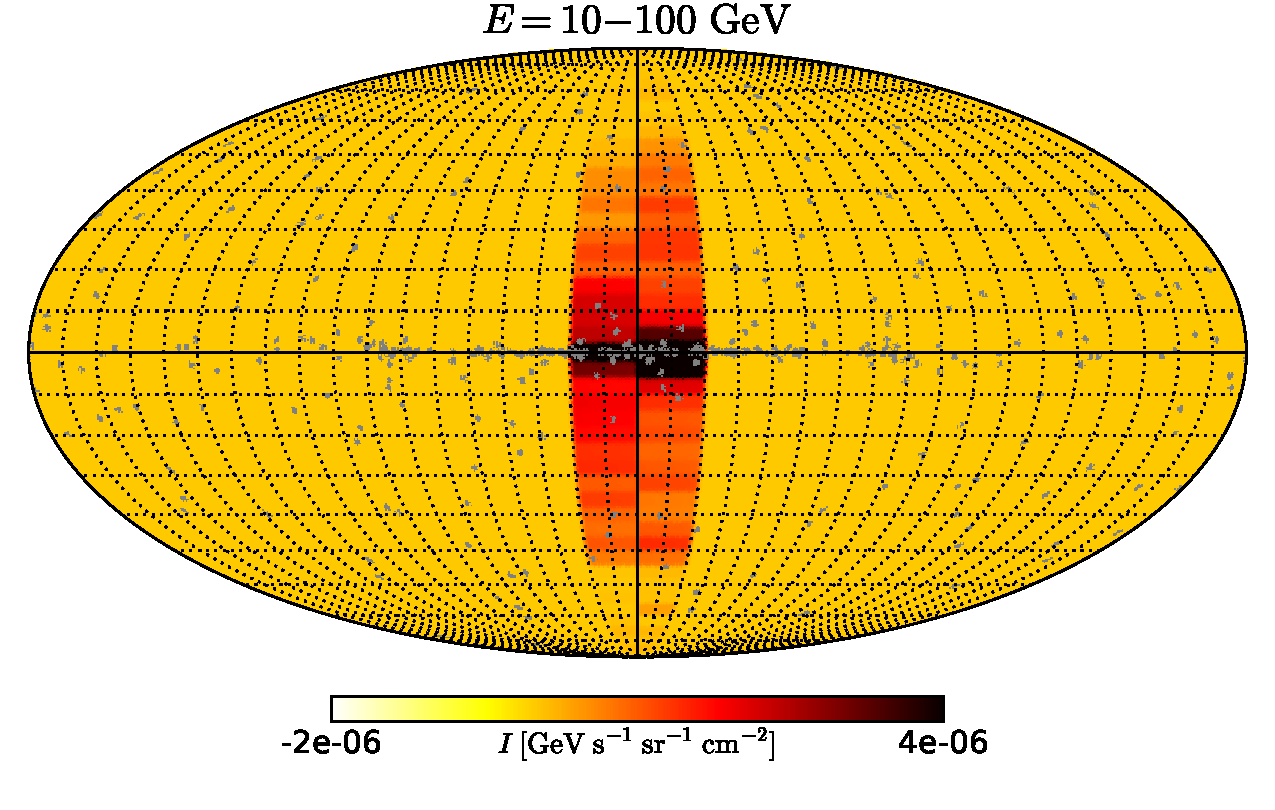
\includegraphics[width=0.45\textwidth]{plots/Mollweide_Boxes_03-10GeV_flux_source_range_1.pdf}\\
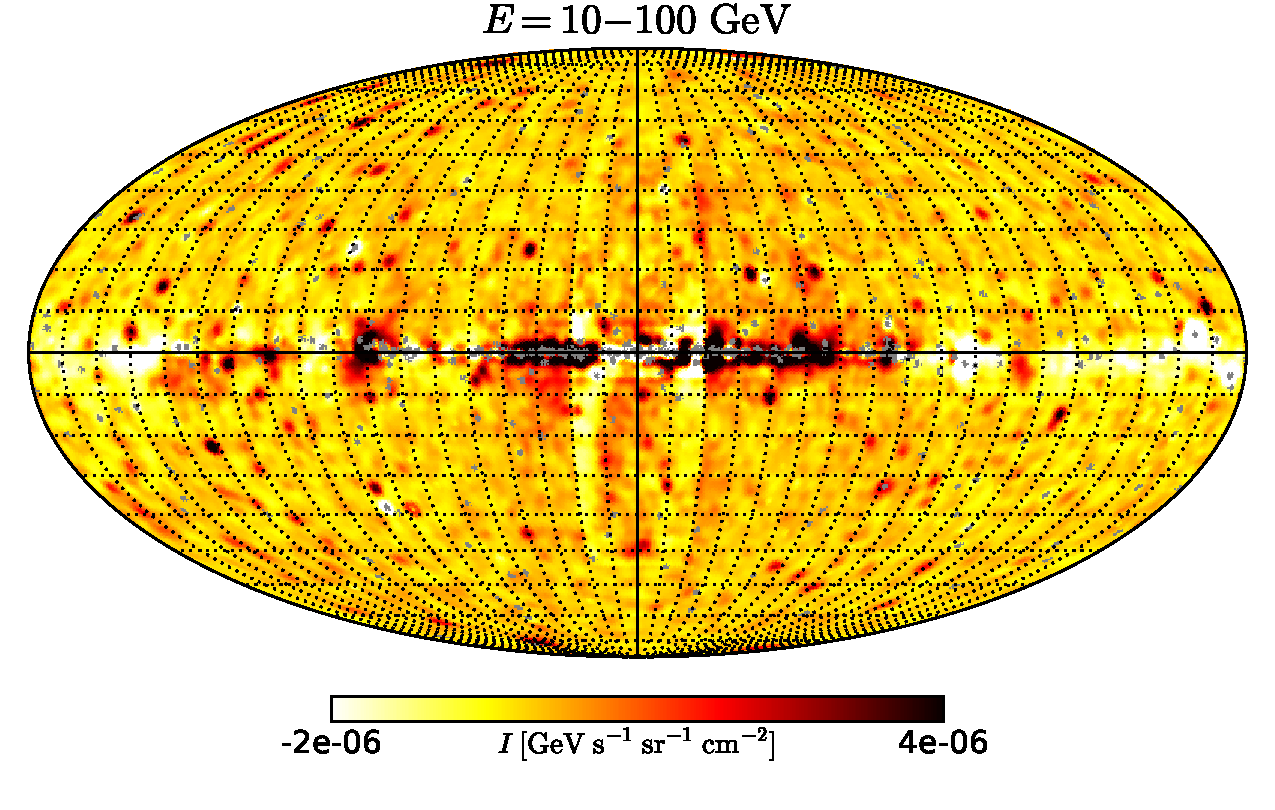
\includegraphics[width=0.45\textwidth]{plots/Mollweide_Boxes_residual_03-10GeV_flux_source_range_1.pdf}
 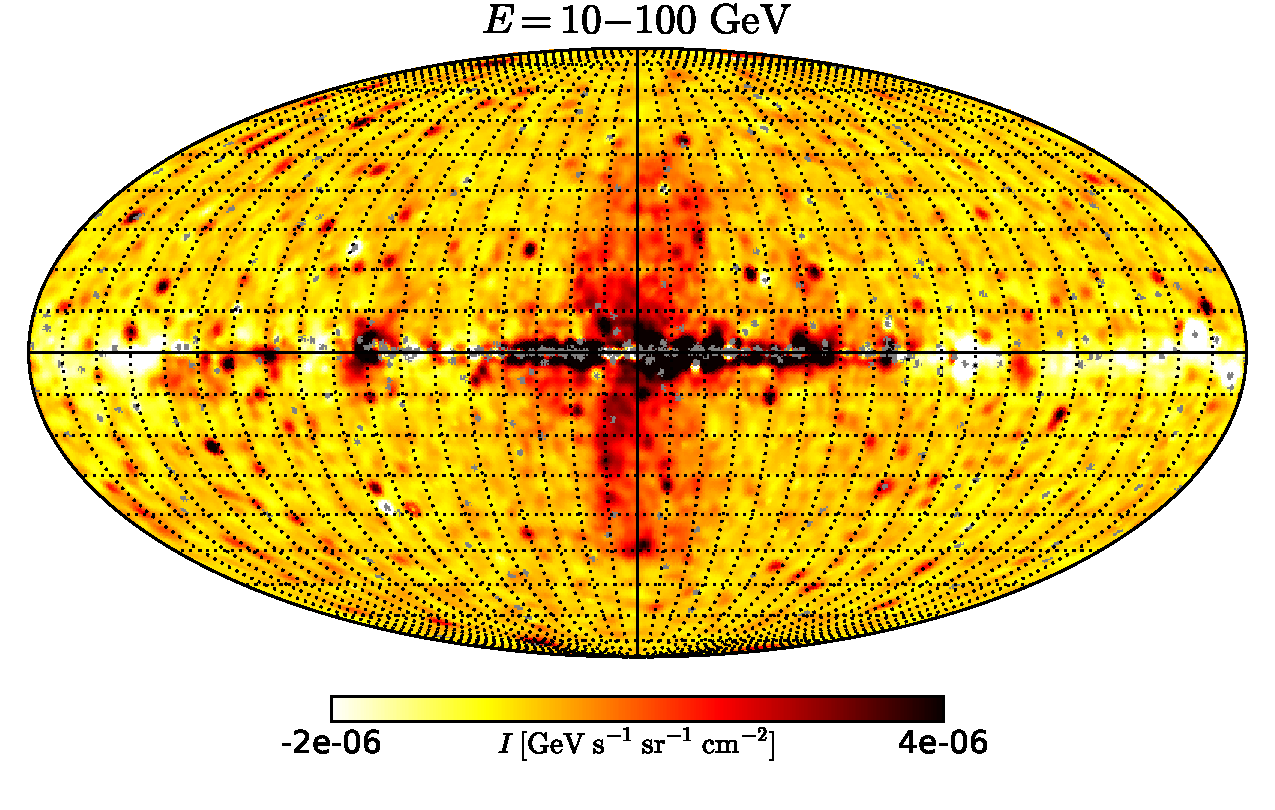
\includegraphics[width=0.45\textwidth]{plots/Mollweide_Boxes_residual+boxes_03-10GeV_flux_source_range_1.pdf}
 \caption{Energy flux of the diffuse model (excluding the rectangles model of the FBs),
 the rectangles model of the FBs, 
the residual after subtracting the total model,
and residuals plus the rectangles model of the FBs
 derived in Section \ref{sec:box_model}
 integrated between 10 and 100 GeV.}
 \label{fig:Maps_Rectangles}
\end{figure}

\subsection{GALPROP model of the foreground and PS refitting}
\label{sec:galprop_model}


\begin{figure}[h]
\centering
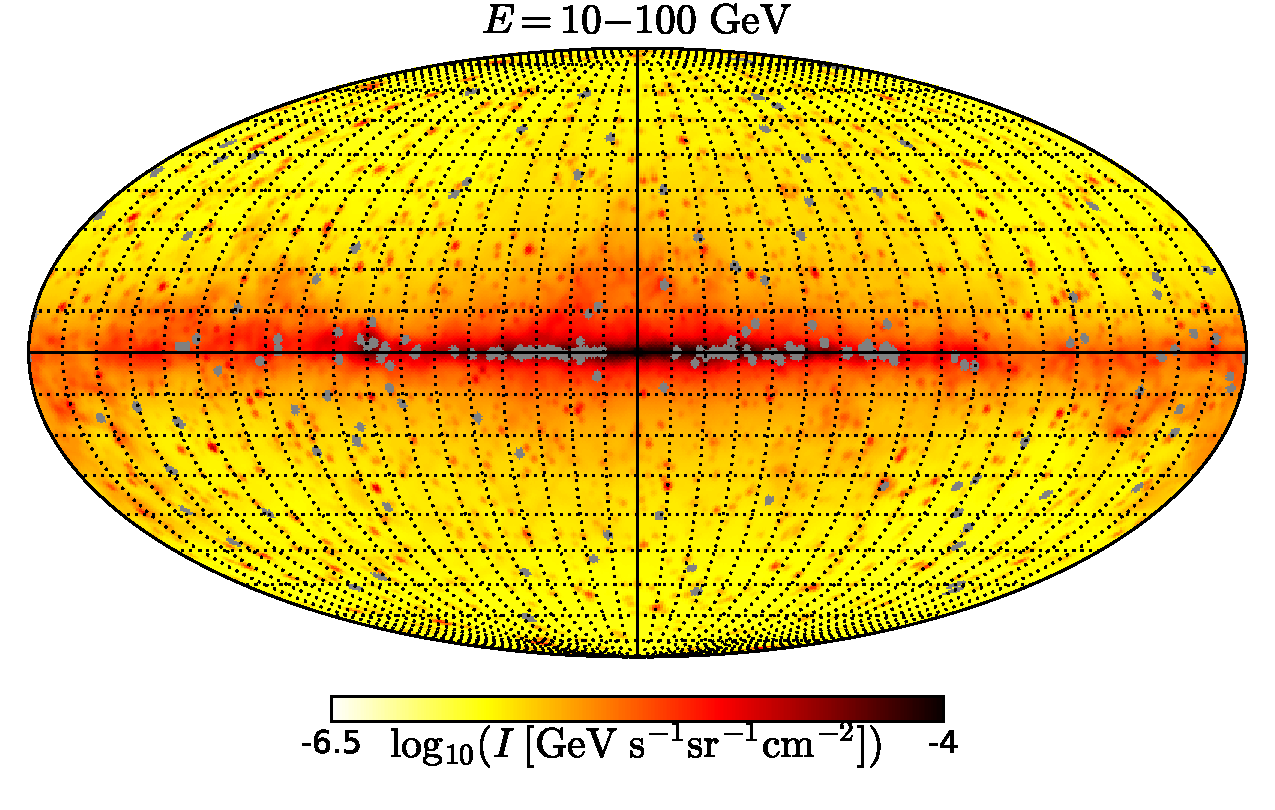
\includegraphics[width=0.45\textwidth]{plots/Mollwiede_GALPROP_model_source_range2_log.pdf}
 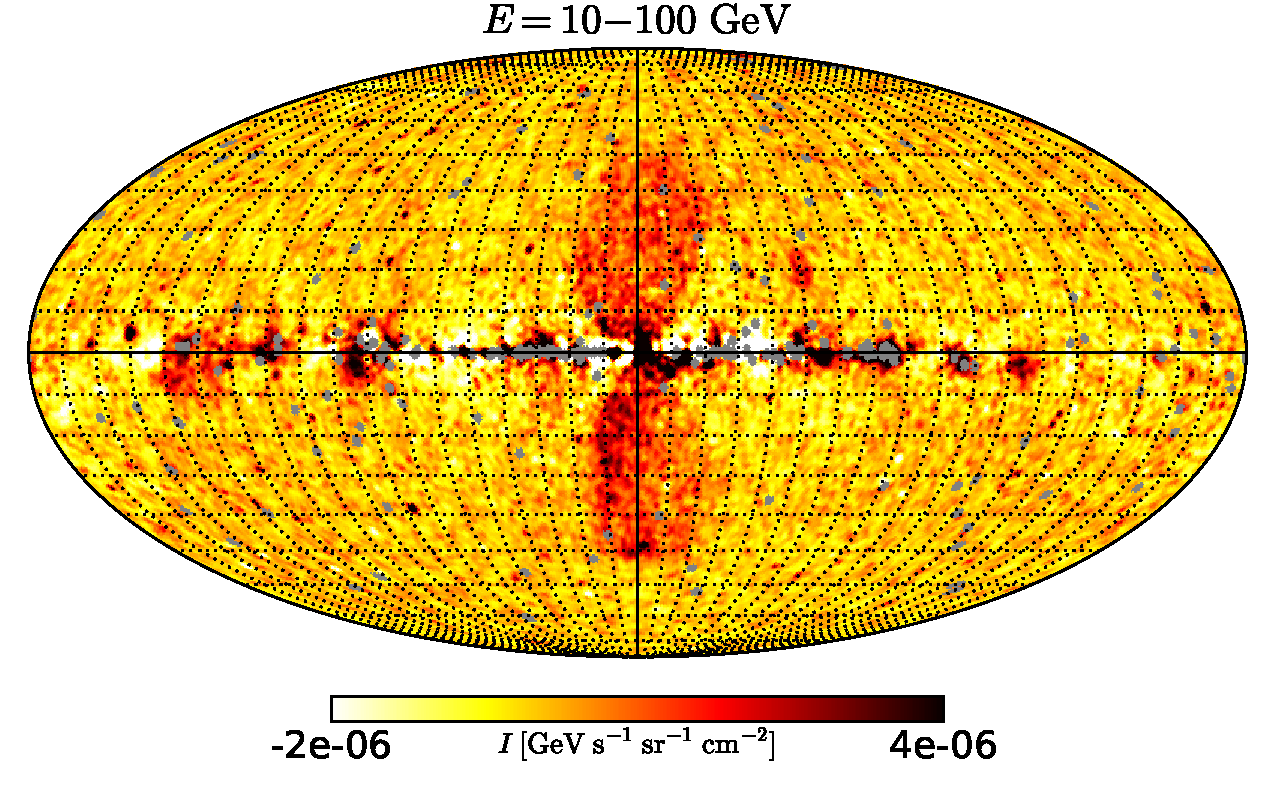
\includegraphics[width=0.45\textwidth]{plots/Mollwiede_GALPROP_source_range2.pdf}
 \caption{Energy flux of the GALPROP background model 
 and of the residuals plus the FBs and the gNFW component derived in Section \ref{sec:galprop_model}
 integrated between 10 and 100 GeV.}
 \label{fig:Maps_GALPROP}
\end{figure}

In this section we fit the gamma-ray data using a model derived with the GALPROP
galactic propagation code v54.1
\citep{Moskalenko:1997gh, Strong:1998fr, Strong:2004de, Ptuskin:2005ax, 2007ARNPS..57..285S, Porter:2008ve,Vladimirov:2010aq}\footnote{\url{http://galprop.stanford.edu}}. 
The model for the diffuse emission components is the same as the Sample model in \cite{2017ApJ...840...43A}.
%The difference is that, within $10^\circ$ from the GC, we do not mask PS and refit 40 PS with largest flux between 10 and 100 GeV.
In particular, we use the GALPROP code to calculate templates for the Galactic diffuse emission components.
We determine 5 templates in each energy bin for gamma rays produced in 
interactions of hadronic CR with gas and bremsstrahlung emission corresponding to 5 Galactocentric rings: 
0 -- 1.5\,kpc, 1.5 -- 3.5\,kpc, and 3.5 -- 8\,kpc; 8 -- 10\,kpc, and 10 -- 50\,kpc.
We assume propagation halo height of 10 kpc, radius of 20 kpc and spin temperature 150 K.
We use 3 inverse Compton templates corresponding to the three ISRF: CMB, 
infrared emission, and starlight.
In addition to GALPROP templates, we use a flat template for the \Fermi bubbles at latitudes $|b| > 10^\circ$~\citep{2014ApJ...793...64A}. 
We model the Loop~I feature using a geometric template \citep[e.g., Figure 2 of][]{2014ApJ...793...64A}
based on a polarization survey at 1.4 GHz~\citep{Wolleben:2007pq}.
The Moon and the Sun \citep{2007Ap&SS.309..359O, 2006ApJ...652L..65M, 2008A&A...480..847O, 2013arXiv1307.0197J} templates 
are obtained with the \Fermi Science Tools%
\footnote{\url{http://fermi.gsfc.nasa.gov/ssc/data/analysis/scitools/solar_template.html}}.
We also include, as a GC excess template, a generalized Navarro-Frenk-White (gNFW) profile with index $\gamma = 1.25$ 
\citep{Goodenough:2009gk,Calore:2014xka,Abazajian:2014fta}
and scaling radius $r_{\rm s} = 20\;{\rm kpc}$.


For the PS, we add sources from the 3FGL catalog~\citep{2015ApJS..218...23A} to form a template
in each energy bin.
We create independent templates for the Large Magellanic cloud and the Cygnus region.
The remaining extended sources are also added in a separate template.
The spatial templates for the extended sources are provided by the 3FGL catalog.
The PS mask in this section is different from the mask that we have used in the previous sections.
We mask the 200 brightest sources outside a $10^\circ$ circle from the GC 
with a radius of $\frac{\delta}{\sqrt{2}} + 1^\circ$ ($\delta = 0\degr\!\!.46$ is the characteristic size of the pixels),
which is larger than the radius of  $\frac{\delta}{\sqrt{2}} + 0^\circ\!\!.5$ used in the previous sections.
Within $10^\circ$ from the GC, we include independent templates for 40 sources with largest flux between 10 and 100 GeV.
In Figure \ref{fig:Maps_GALPROP} we show the residual emission plus the \Fermi bubbles model and the gNFW model summed over energies between 10 and 100 GeV.
Due to more free parameters in this model in the Galactic plane relative to the models considered in the previous sections,
there are fewer positive residuals in the Galactic plane.
There are, however, negative residuals in several locations, which signals about deficiencies in the model. 
In particular, there is a rather significant negative residual to the east of the GC.
Nonetheless, the FBs are clearly visible as well as the bright emission at the base of the FBs which also displays a shift to negative
longitudes relative to the GC.


